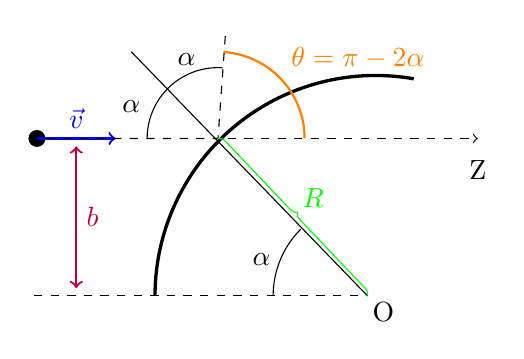
\begin{tikzpicture}
\usetikzlibrary{decorations.pathreplacing}
\draw  [fill] (-2.3,1.5) node (v1) {} circle (0.1);
\draw [blue, ->, thick] (v1.center) -- (-1.3,1.5)node [midway, above]{$\vec{v}$};
\draw [dashed] (v1) -- (0,1.5) node (v3) {} -- (0.1,2.9);
\draw (1.9,-0.5) node (v4) {} -- (-1.1,2.6);
\node at (2.1,-0.7) {O};


\draw [dashed,->] (v3) -- (3.3,1.5);


\draw (-0.9,1.5) arc (180:86.4:0.9);
\node at (-1.1,1.9) {$\alpha$};
\node at (-0.4,2.5) {$\alpha$};



\draw [very thick] (-0.8,-0.5) node (v2) {} arc (180:80:2.8);

\draw [orange, thick] (0.0691,2.5978) arc (86.3983:0:1.1)node [midway, above right]{$\theta=\pi-2\alpha$};
\draw [dashed](v4) -- (-2.4,-0.5);
\draw [purple, <->, thick] (-1.8,1.4) -- (-1.8,-0.4)node [midway, right]{$b$};
\draw (0.7,-0.5) arc (180:135:1.2)node [midway, left]{$\alpha$};
\node at (3.3,1.1) {Z};

\draw [decorate, decoration=brace, draw=green] (v3.center)--(v4.center) node [midway,above right,green] {$R$};
\end{tikzpicture}